% couvertures-python.tex -- couvertures de l'edition Python : les pages
% scannees de couvertures-aplaties.pdf (edition OCaml), ou l'on remplace
% "OCaml" par "Python" (couverture, page de titre, 4e de couverture) et
% "(if,match)" par "(if, elif)" (4e de couverture) : un rectangle de la
% couleur du fond cache l'ancien mot, le nouveau est ecrit par-dessus.
% Coordonnees en points PDF de la page A4 (origine en bas a gauche).
%   pdflatex couvertures-python ; pdflatex couvertures-python
\documentclass{article}
\usepackage[a4paper,margin=0pt]{geometry}
\usepackage[T1]{fontenc}
\usepackage{pdfpages}
\usepackage{tikz}
\usepackage{graphicx}
\definecolor{bleucouv}{RGB}{33,80,117}
\definecolor{blanccouv}{RGB}{245,247,241}
\definecolor{bleudos}{RGB}{32,70,102}
\definecolor{blancdos}{RGB}{205,210,208}
\newcommand\ici[2]{([xshift=#1bp,yshift=#2bp]current page.south west)}
\begin{document}
% 1 : couverture
\includepdf[pages=1,pagecommand={\thispagestyle{empty}%
  \begin{tikzpicture}[remember picture,overlay]
    \fill[bleucouv] \ici{152}{568} rectangle \ici{278}{607};
    \node[anchor=base west,inner sep=0,text=blanccouv] at \ici{154}{572.9}
      {\scalebox{0.86}[1]{\fontsize{44.5}{44.5}\usefont{T1}{phv}{b}{sl}Python}};
  \end{tikzpicture}}]{couvertures-aplaties.pdf}
\includepdf[pages=2]{couvertures-aplaties.pdf}
% 3 : page de titre
\includepdf[pages=3,pagecommand={\thispagestyle{empty}%
  \begin{tikzpicture}[remember picture,overlay]
    \fill[white] \ici{162}{564} rectangle \ici{272}{595};
    \node[anchor=base west,inner sep=0,text=black] at \ici{165}{570.5}
      {\scalebox{0.86}[1]{\fontsize{37}{37}\usefont{T1}{phv}{m}{sl}Python}};
  \end{tikzpicture}}]{couvertures-aplaties.pdf}
\includepdf[pages=4-5]{couvertures-aplaties.pdf}
% 6 : 4e de couverture
\includepdf[pages=6,pagecommand={\thispagestyle{empty}%
  \begin{tikzpicture}[remember picture,overlay]
    \fill[bleudos] \ici{233.5}{651.5} rectangle \ici{265.5}{664};
    \node[anchor=base west,inner sep=0,text=blancdos] at \ici{235.5}{654.5}
      {\fontsize{11.3}{11.3}\usefont{T1}{phv}{mc}{n}Python};
    \fill[bleudos] \ici{121}{615.5} rectangle \ici{186.5}{628};
    \node[anchor=base west,inner sep=0,text=blancdos] at \ici{122.5}{619.5}
      {\fontsize{10}{10}\usefont{T1}{pcr}{b}{n}(if,elif),};
  \end{tikzpicture}}]{couvertures-aplaties.pdf}
\end{document}
